\documentclass{article}
\usepackage[margin=1in]{geometry}
\usepackage{amsmath,amsthm,amssymb}
\usepackage{bbm,enumerate,mathtools}
\usepackage{tikz,pgfplots}
\usepackage{chessboard}
\usepackage[hidelinks]{hyperref}
\usepackage{multicol} % Problem 35

\newenvironment{question}{\begin{trivlist}\item[\textbf{Question.}]}{\end{trivlist}}
\newenvironment{note}{\begin{trivlist}\item[\textbf{Note.}]}{\end{trivlist}}
\newenvironment{references}{\begin{trivlist}\item[\textbf{References.}]}{\end{trivlist}}
\newenvironment{related}{\begin{trivlist}\item[\textbf{Related.}]\end{trivlist}\begin{enumerate}}{\end{enumerate}}


\begin{document}
\rating{2}{3}
Consider an $n$-coloring of a triangular grid such that no sub-triangle has
corners all with the same color.\\\vspace{0.5cm}
\begin{figure}[!h]
  \centering
  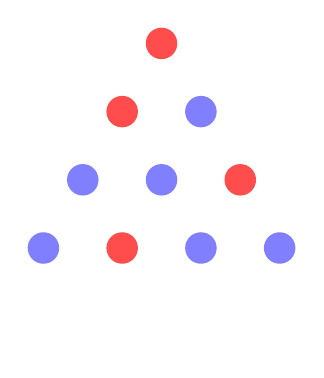
\begin{tikzpicture}
    \fill[blue!50] (0, 0) circle (0.2cm);
    \fill[red!70]  (1, 0) circle (0.2cm);
    \fill[blue!50] (2, 0) circle (0.2cm);
    \fill[blue!50] (3, 0) circle (0.2cm);
    \fill[blue!50] (0 + 0.5, {1 * sqrt(3)/2}) circle (0.2cm);
    \fill[blue!50] (1 + 0.5, {1 * sqrt(3)/2}) circle (0.2cm);
    \fill[red!70]  (2 + 0.5, {1 * sqrt(3)/2}) circle (0.2cm);
    \fill[red!70]  (0 + 1, {2 * sqrt(3)/2}) circle (0.2cm);
    \fill[blue!50] (1 + 1, {2 * sqrt(3)/2}) circle (0.2cm);
    \fill[red!70]  (0 + 1.5, {3 * sqrt(3)/2}) circle (0.2cm);
    \draw[white] (0,-1.28)--(0,-1.28);
  \end{tikzpicture} \hspace{1cm} 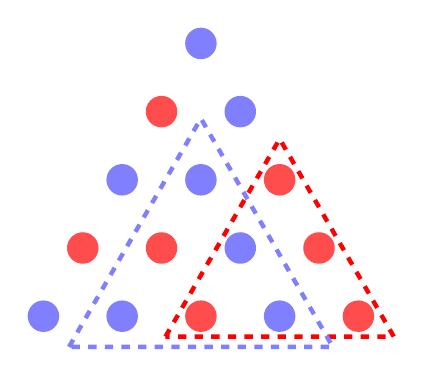
\begin{tikzpicture}
    \fill[blue!50] (0, 0) circle (0.2cm);
    \fill[blue!50] (1, 0) circle (0.2cm);
    \fill[red!70]  (2, 0) circle (0.2cm);
    \fill[blue!50] (3, 0) circle (0.2cm);
    \fill[red!70]  (4, 0) circle (0.2cm);
    \fill[red!70]  (0 + 0.5, {1 * sqrt(3)/2}) circle (0.2cm);
    \fill[red!70]  (1 + 0.5, {1 * sqrt(3)/2}) circle (0.2cm);
    \fill[blue!50] (2 + 0.5, {1 * sqrt(3)/2}) circle (0.2cm);
    \fill[red!70]  (3 + 0.5, {1 * sqrt(3)/2}) circle (0.2cm);
    \fill[blue!50] (0 + 1, {2 * sqrt(3)/2}) circle (0.2cm);
    \fill[blue!50] (1 + 1, {2 * sqrt(3)/2}) circle (0.2cm);
    \fill[red!70]  (2 + 1, {2 * sqrt(3)/2}) circle (0.2cm);
    \fill[red!70]  (0 + 1.5, {3 * sqrt(3)/2}) circle (0.2cm);
    \fill[blue!50] (1 + 1.5, {3 * sqrt(3)/2}) circle (0.2cm);
    \fill[blue!50] (0 + 2, {4 * sqrt(3)/2}) circle (0.2cm);

    % \foreach \t in {1.5} {
    \def\t {1.3};
    \draw[red, ultra thick, dashed]
      ({2 + (1 - \t) * 1.5}, {(1 - \t) * sqrt(3)/2})--
      ({2 + (1 - \t) * 1 + \t * 1}, {\t * sqrt(3)})--
      ({2 + (1 - \t) * 0.5 + \t * 2}, {(1 - \t) * sqrt(3)/2})--
      ({2 + (1 - \t) * 1.5}, {(1 - \t) * sqrt(3)/2});

      \def\t {1.45};
      \draw[blue!50, ultra thick, dashed]
        ({1 + (1 - \t) * 1.5}, {(1 - \t) * sqrt(3)/2})--
        ({1 + (1 - \t) * 1 + \t * 1}, {\t * sqrt(3)})--
        ({1 + (1 - \t) * 0.5 + \t * 2}, {(1 - \t) * sqrt(3)/2})--
        ({1 + (1 - \t) * 1.5}, {(1 - \t) * sqrt(3)/2});
    \end{tikzpicture}
    \caption{
      On the left is an example of a triangle on two labels that has no
      sub-triangles with equal corners. On the right is a non-example of such a
      triangle on two labels: it has two sub-triangles with equal corners.
    }
\end{figure}

\begin{question}
  Given $n$ labels, what is the biggest triangle that can be constructed?
  Call the side length of such a triangle $a(n)$.
\end{question}
\begin{related}
  \item Given an $n$-coloring of a triangle of side length $k$, what number
    of sub-triangles with equal corners must exist?
  \item How many such triangles exist?
  \item What if diagonal equilateral triangles also are not allowed to have equal corners?
  \item What if this is done with hexagons instead of triangles?
  \item What if this is done on a square grid?
  \item What if for $n \geq 3$ no \textit{two} corners are allowed to be equal?
    (This is a bit like a peaceable queens problem on a hexagonal chessboard.)
\end{related}
\begin{references}
  \item \url{https://math.stackexchange.com/a/2416790/121988}
  \item \url{https://math.stackexchange.com/a/2636168/121988}
\end{references}
\end{document}
